Mauris pharetra et ultrices neque ornare aenean. Nascetur ridiculus mus mauris vitae ultricies. Placerat orci nulla pellentesque dignissim enim sit amet. Quis risus sed vulputate odio ut. Semper feugiat nibh sed pulvinar proin gravida hendrerit lectus. Nec feugiat nisl pretium fusce id velit ut tortor.


\section{Section of Theory}

Two different coordinate systems are used in ship manoeuvring. A ship-fixed coordinate system (\textit{oxyz}), fixed to the hull at the origin ($o$) and a space-fixed (\emph{inertial}) coordinate system (\textit{OXYZ}). For consistency with the experimental data available, the origin for the ship-fixed coordinate system is taken at midship, and not at the centre of gravity, for all simulations presented herein. The motions of the ship-fixed coordinate system are expressed relative to the space-fixed coordinate system. 

\begin{figure}[H]
	\centering
	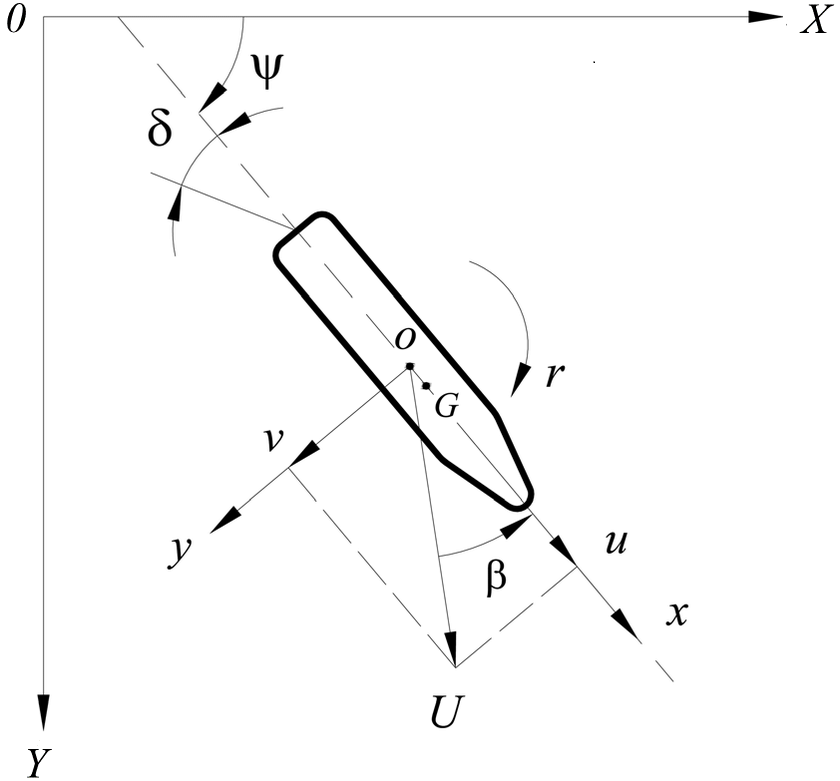
\includegraphics[width=0.48\linewidth]{Cxyz.png}
	% part in the [] goes to list of table, part in {} goes to text
	\caption[Space and ship-fixed coordinate system.]{Space and ship-fixed coordinate system. Adapted from \citet{luo2016parameter}.}
	\label{fig:cxyz}
\end{figure}
In the ship-fixed coordinate system, \textit{x} is pointing forward, \textit{y} to starboard and \textit{z} downwards. The origin of the space-fixed coordinate system is usually taken as lying on the undisturbed free surface.  A positive yaw angle $\psi$ is therefore defined as a \emph{clockwise} rotation of the ship in the space-fixed coordinate system. Similarly, a positive drift angle $\beta$ corresponds to the flow coming from starboard.